% Options for packages loaded elsewhere
\PassOptionsToPackage{unicode}{hyperref}
\PassOptionsToPackage{hyphens}{url}
%
\documentclass[
  12pt,
]{article}
\usepackage{amsmath,amssymb}
\usepackage{iftex}
\ifPDFTeX
  \usepackage[T1]{fontenc}
  \usepackage[utf8]{inputenc}
  \usepackage{textcomp} % provide euro and other symbols
\else % if luatex or xetex
  \usepackage{unicode-math} % this also loads fontspec
  \defaultfontfeatures{Scale=MatchLowercase}
  \defaultfontfeatures[\rmfamily]{Ligatures=TeX,Scale=1}
\fi
\usepackage{lmodern}
\ifPDFTeX\else
  % xetex/luatex font selection
\fi
% Use upquote if available, for straight quotes in verbatim environments
\IfFileExists{upquote.sty}{\usepackage{upquote}}{}
\IfFileExists{microtype.sty}{% use microtype if available
  \usepackage[]{microtype}
  \UseMicrotypeSet[protrusion]{basicmath} % disable protrusion for tt fonts
}{}
\makeatletter
\@ifundefined{KOMAClassName}{% if non-KOMA class
  \IfFileExists{parskip.sty}{%
    \usepackage{parskip}
  }{% else
    \setlength{\parindent}{0pt}
    \setlength{\parskip}{6pt plus 2pt minus 1pt}}
}{% if KOMA class
  \KOMAoptions{parskip=half}}
\makeatother
\usepackage{xcolor}
\usepackage[margin=1in]{geometry}
\usepackage{graphicx}
\makeatletter
\def\maxwidth{\ifdim\Gin@nat@width>\linewidth\linewidth\else\Gin@nat@width\fi}
\def\maxheight{\ifdim\Gin@nat@height>\textheight\textheight\else\Gin@nat@height\fi}
\makeatother
% Scale images if necessary, so that they will not overflow the page
% margins by default, and it is still possible to overwrite the defaults
% using explicit options in \includegraphics[width, height, ...]{}
\setkeys{Gin}{width=\maxwidth,height=\maxheight,keepaspectratio}
% Set default figure placement to htbp
\makeatletter
\def\fps@figure{htbp}
\makeatother
\setlength{\emergencystretch}{3em} % prevent overfull lines
\providecommand{\tightlist}{%
  \setlength{\itemsep}{0pt}\setlength{\parskip}{0pt}}
\setcounter{secnumdepth}{5}
\usepackage{setspace,lscape} \usepackage{amsmath} \usepackage{array} \usepackage{caption,subcaption} \usepackage{longtable} \usepackage{booktabs} \usepackage{enumitem} \usepackage{standalone} \renewcommand{\arraystretch}{1.5} \captionsetup[table]{skip=5pt} \setstretch{1.5}
\ifLuaTeX
  \usepackage{selnolig}  % disable illegal ligatures
\fi
\usepackage[]{natbib}
\bibliographystyle{apalike}
\IfFileExists{bookmark.sty}{\usepackage{bookmark}}{\usepackage{hyperref}}
\IfFileExists{xurl.sty}{\usepackage{xurl}}{} % add URL line breaks if available
\urlstyle{same}
\hypersetup{
  pdftitle={Results of Experiment 2},
  pdfauthor={Zijian Zark Wang},
  hidelinks,
  pdfcreator={LaTeX via pandoc}}

\title{Results of Experiment 2}
\author{Zijian Zark Wang}
\date{April 17, 2024}

\begin{document}
\maketitle

\hypertarget{experiment-3-causal-manipulation-of-attention}{%
\section{Experiment 3: Causal Manipulation of
Attention}\label{experiment-3-causal-manipulation-of-attention}}

\hypertarget{procedure}{%
\subsection{Procedure}\label{procedure}}

We recruited 300 UK residents via Prolific. Participants are asked to
complete a series of choice tasks. At each time there is only one task
presented on the screen. These tasks are divided into four parts. Before
each part begins, there are 2-3 example tasks to help participants get
familiarized with the tasks in the corresponding part.

In Part 1-2, each choice is between a single immediate monetary reward
and a sequence of two monetary rewards. Participants have to choose the
option they prefer.

\begin{figure}
  \centering
  \begin{subfigure}{\textwidth}
    \centering
    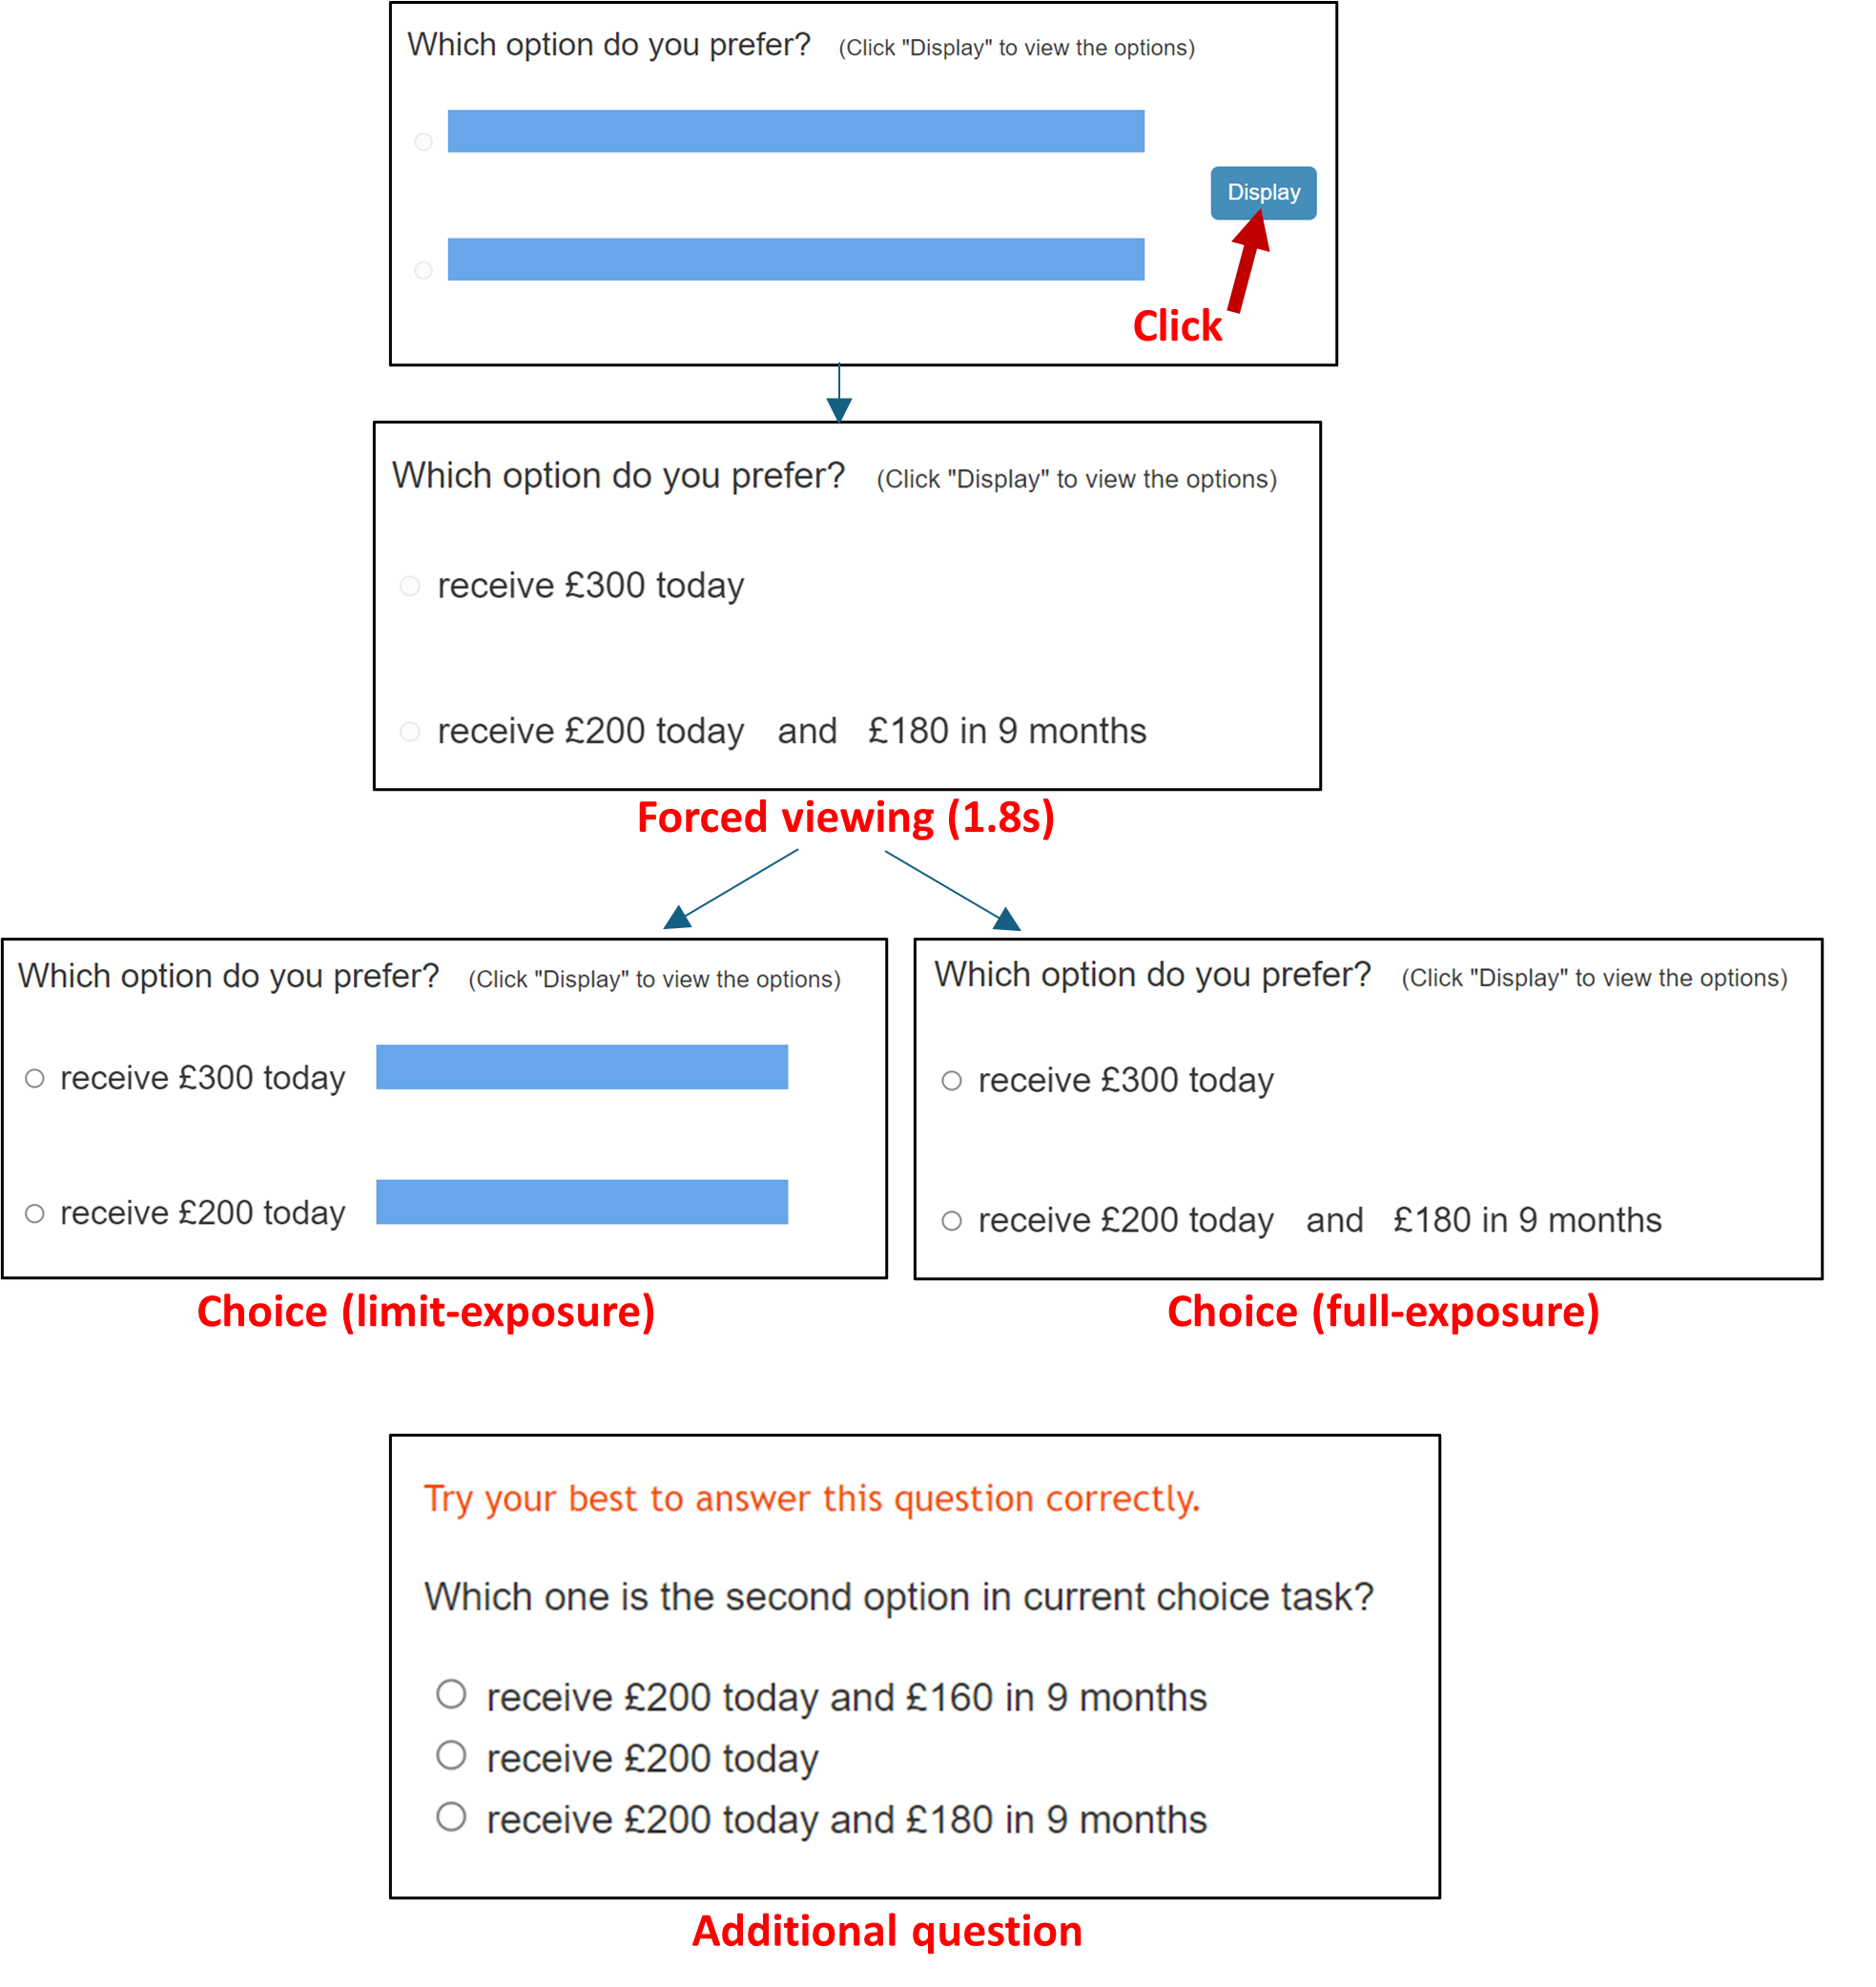
\includegraphics[width=\linewidth]{figures/exp3_intertemporal_task.png}
    \subcaption{Intertemporal Choice Task}
  \end{subfigure}
  \begin{subfigure}{\textwidth}
    \vspace{2em}
    \centering
    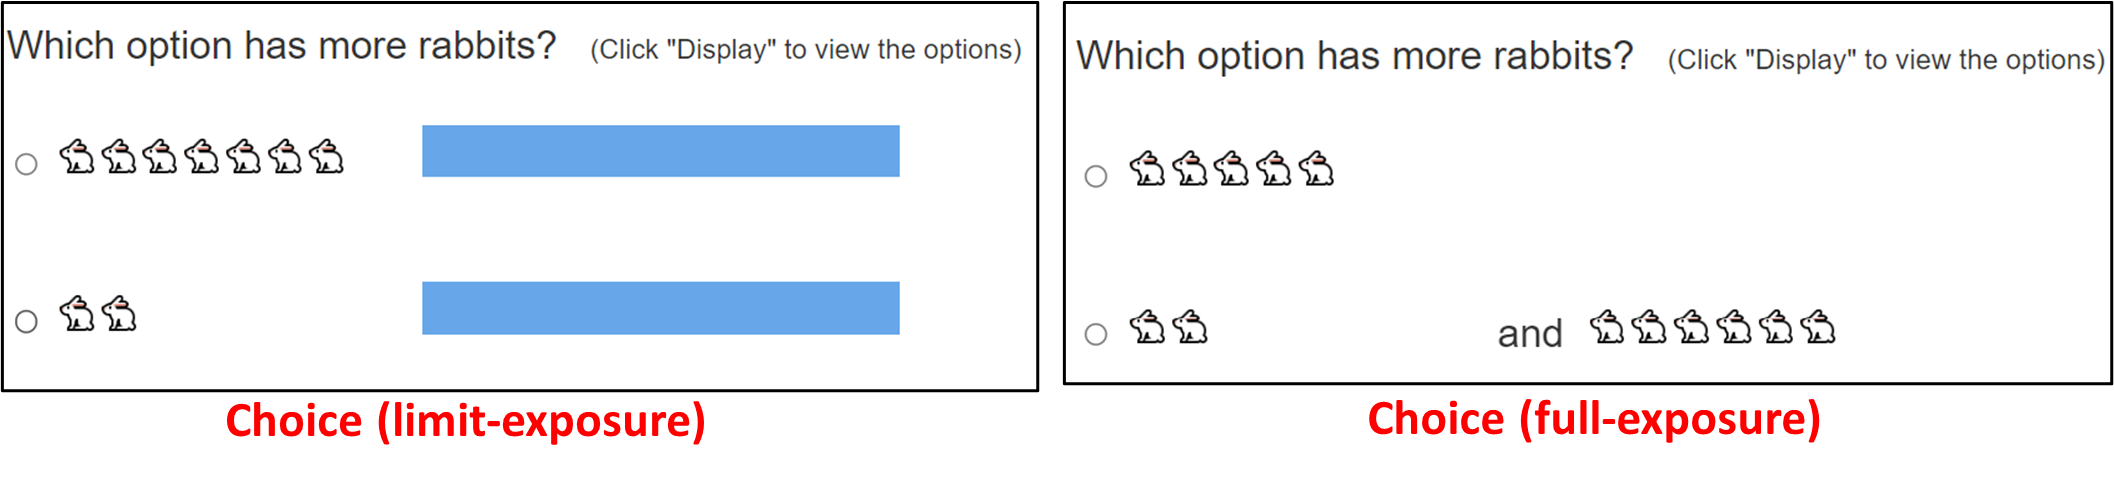
\includegraphics[width=\linewidth]{figures/exp3_rabbit_task.png}
    \subcaption{Count-the-Rabbits Task}
  \end{subfigure}
  \caption{Screenshot of Experiment 3}
  \label{fig:exp3_screenshot}
\end{figure}


\documentclass[12pt]{article}


\begin{document}
\begin{table}
    \caption{Regression Results for Intertemporal Choice Tasks}
    \vspace*{12pt}
    \centering

      \begin{tabular}{llll}
\hline
 & (1) Pooled & (2) FE & (3) FE \\
\hline
Group & 0.082 & 0.034 & -0.1 \\
 & (0.189) & (0.102) & (0.096) \\
Question$\cdot1\{\text{Group}=0\}$ & 0.084 & 0.289 & 0.289 \\
 & (0.059) & (0.185) & (0.183) \\
Question$\cdot1\{\text{Group}=1\}$ & 0.223$^{***}$ & 0.535$^{***}$ & 0.535$^{***}$ \\
 & (0.067) & (0.162) & (0.161) \\
$1\{\rho=0.2\}$ & -0.276$^{***}$ & -0.756$^{***}$ & -0.756$^{***}$ \\
 & (0.051) & (0.135) & (0.133) \\
$1\{\rho=0.3\}$ & -0.333$^{***}$ & -0.915$^{***}$ & -0.915$^{***}$ \\
 & (0.059) & (0.156) & (0.155) \\
$1\{\rho=0.4\}$ & -0.254$^{***}$ & -0.688$^{***}$ & -0.688$^{***}$ \\
 & (0.061) & (0.166) & (0.164) \\
$1\{\rho=0.5\}$ & -0.193$^{**}$ & -0.516$^{**}$ & -0.516$^{**}$ \\
 & (0.071) & (0.194) & (0.192) \\
$1\{\rho=0.6\}$ & -0.468$^{***}$ & -1.281$^{***}$ & -1.281$^{***}$ \\
 & (0.081) & (0.22) & (0.218) \\
$1\{s=240\}$ & 0.191$^{***}$ & 0.53$^{***}$ & 0.53$^{***}$ \\
 & (0.044) & (0.119) & (0.118) \\
$1\{s=280\}$ & 0.665$^{***}$ & 1.795$^{***}$ & 1.795$^{***}$ \\
 & (0.058) & (0.126) & (0.125) \\
$1\{s=320\}$ & 0.475$^{***}$ & 1.293$^{***}$ & 1.293$^{***}$ \\
 & (0.053) & (0.124) & (0.123) \\\hline

observations & 7056 & 4416 & 7056 \\
aic & 9621.97 & 4294.947 & 4303.619 \\
\hline
\end{tabular}
% INSERT reg_choice

    \vspace*{4pt}
    \centering
    \begin{minipage}{0.85\textwidth}
    {\par\footnotesize Note: * $p<0.05$, ** $p<0.01$, *** $p<0.001$. Standard errors are clustered at the subject level and are reported in the parentheses. The p-values are calculated based on Wald tests. FE denotes fixed effects. Subject-specific dummies are omitted in this table.}
    \end{minipage}
    \label{tab:manipulate_intertemporal_choice}
\end{table}

\end{document}




\documentclass[12pt]{article}


\begin{document}
\begin{table}
    \caption{Regression Results for Count-the-Rabbits Tasks}
    \vspace*{12pt}
    \centering

      \begin{tabular}{lllll}
\hline
 & (1) Pooled & (2) FE & (3) FE & (4) FE \\
\hline
Group & -0.73$^{*}$ & -4.379$^{***}$ & -0.158 & -0.757 \\
 & (0.33) & (1.114) & (8.618) & (0.392) \\
Question$\cdot1\{\text{Group}=0\}$ & 0.574$^{*}$ & 1.378$^{*}$ & 1.56$^{*}$ & 2.005$^{**}$ \\
 & (0.226) & (0.6) & (0.689) & (0.744) \\
Questsion$\cdot1\{\text{Group}=1\}$ & 0.062 & 0.152 & 0.391 & 0.145 \\
 & (0.318) & (0.368) & (0.422) & (0.344) \\
$1\{r_2 + r_3 > r_1\}$ & 7.797$^{***}$ & 11.71$^{***}$ & 11.198$^{***}$ & 6.181$^{***}$ \\
 & (0.377) & (1.091) & (1.249) & (0.552) \\
$1\{r_2 =2\}$ & 0.106 & 0.183 & 0.161 & 0.217 \\
 & (0.274) & (0.378) & (0.45) & (0.393) \\
$1\{r_2=3\}$ & -0.655$^{***}$ & -0.95$^{**}$ & -1.014$^{*}$ & -0.991$^{***}$ \\
 & (0.228) & (0.338) & (0.395) & (0.35) \\
$1\{r_1=8\}$ & 0.145 & 0.192 & 0.145 & 0.191 \\
 & (0.166) & (0.241) & (0.272) & (0.252) \\\hline

observations & 3504 & 3504 & 2190 & 810 \\
aic & 878.752 & 1100.636 & 746.754 & 583.857 \\
\hline
\end{tabular}
% INSERT reg_rabbit

    \vspace*{4pt}
    \centering
    \begin{minipage}{0.85\textwidth}
    {\par\footnotesize Note: * $p<0.05$, ** $p<0.01$, *** $p<0.005$. Standard errors are clustered at the subject level and are reported in the parentheses. The p-values are calculated based on Wald tests. FE denotes individual fixed-effects. Model (1)-(2) are run upon the full sample, (3) is for those having changed choices at least once in intertemporal choice tasks, (4) is for those having made wrong choices in count-the-rabbits tasks. Intercepts and subject-specific dummies are omitted in this table.}
    \end{minipage}
    \label{tab:exp3_reg_rabbit_choice}
\end{table}

\end{document}




\begin{table}[!h]
    \caption{Predicting response times with choices and conditions in Experiment 1}
    \vspace*{10pt}
    \centering

      \begin{tabular}{lll}
\hline
 & Intertemporal Choice & Count-the-Rabbits \\
\hline
Group & -0.684$^{***}$ & -0.792$^{***}$ \\
 & (0.141) & (0.144) \\
Question$\cdot1\{\text{Group}=0\}$ & -0.165 & 0.912$^{***}$ \\
 & (0.174) & (0.199) \\
Question$\cdot1\{\text{Group}=1\}$ & 0.457$^{***}$ & 0.849$^{***}$ \\
 & (0.101) & (0.132) \\
Choice & 0.954$^{*}$ & 1.291$^{***}$ \\
 & (0.399) & (0.456) \\
Choice$\times$Group & -0.762$^{*}$ & -1.265$^{***}$ \\
 & (0.304) & (0.229) \\
Choice$\times$Question$\cdot1\{\text{Group}=0\}$ & 0.001 & -0.138 \\
 & (0.257) & (0.23) \\
Choice$\times$Question$\cdot1\{\text{Group}=1\}$ & -0.12 & 0.263 \\
 & (0.195) & (0.175) \\\hline

observations & 4393 & 2179 \\
AIC & 18560.034 & 8711.872 \\
adj-$R^2$ & 0.381 & 0.55 \\
\hline
\end{tabular}
% INSERT reg_response_time

    \vspace*{4pt}
    \centering
    \begin{minipage}{0.85\textwidth}
    {\par\footnotesize Note: * $p<0.05$, ** $p<0.01$, *** $p<0.005$. Both models are estimated through 2SLS method. For first-stage regression, we use the model for Column (2) in Table \ref{tab:exp3_reg_intertemporal_choice} to predict intertemporal choices, and the model for Column (3) in Table \ref{tab:exp3_reg_rabbit_choice} to predict count-the-rabbits choices. The variable Choice which is 1 if the predicted choice is the sequence option and is 0 otherwise. For second-stage regression, indepdent variables are the predictors shown in the table plus task-specific dummies and their interactions with Choice, and participant-specific dummies. Standard errors (in the parentheses) are clustered at the subject level. $p$-values are calculated based on t-tests. }
    \end{minipage}
    \label{tab:exp3_reg_response_time}
\end{table}




\renewcommand\refname{Reference}
  \bibliography{experiment-2-ref.bib}

\end{document}
